\documentclass[a4paper,12pt]{article}
\usepackage[utf8]{inputenc}
\usepackage{graphicx}
\usepackage{fancyhdr}
\usepackage{amsmath}
\usepackage{adjustbox}
\usepackage{mathtools}
\usepackage{float}
\usepackage[spanish]{babel} 
\usepackage{lastpage}
\usepackage{amssymb} % Para símbolos matemáticos adicionales
\usepackage{hyperref}
\usepackage{cleveref}
%\usepackage[none]{hyphenat}
\usepackage{array}

\usepackage{multirow}
\usepackage{textcomp}
\usepackage[left=2.5cm, right=2.5cm, top=3cm, bottom=3cm]{geometry}

\graphicspath{{Imagenes/}}

% Encabezado y pie de página
\pagestyle{fancy}
\fancyhf{}
\setlength{\headheight}{30 pt}
\renewcommand{\headrulewidth}{0.2pt}
\fancyhead[R]{\begin{tabular}{@{}l@{}}
\includegraphics[scale=0.4]{escudo.PNG}\end{tabular}}
\fancyhead[L]{\begin{tabular}{@{}c@{}} \textbf{Robótica I - Año: 2024} \\ Trabajo Práctico 3: Denavit y Hartenberg \end{tabular}}


\fancyfoot[R]{\thepage}
\fancyfoot[C]{\begin{tabular}{@{}c@{}}\textbf{BORQUEZ PEREZ Juan Manuel}\\ \textbf{RAYES CANO Julían Andrés}\end{tabular}}
\renewcommand{\footrulewidth}{0.2pt}

\begin{document}

\begin{titlepage}
    \centering
    \vspace*{5cm}
    {\Huge\bfseries Informe de Trabajo Práctico N°3}\\
    \vspace{0.2cm}
    {\Large \textbf{Ejercicio Obligatorio}}\\
    \vspace{0.5cm}
    {\Large \textbf{Denavit y Hartenberg}}\\
    \vspace{0.5cm}
    {\Large Robótica I}\\
    \vspace{0.5 cm}
    {\Large Ingeniería en Mecatrónica}\\
    \vspace{0.2 cm}
    {\Large Facultad de Ingeniería - UNCUYO}\\
    \vspace{1.5cm}
    Juan Manuel BORQUEZ PEREZ\\
    Julián Andrés RAYES CANO\\
    \vfill
    {\begin{tabular}{@{}c@{}}
\includegraphics[scale=0.4]{escudo.PNG}\end{tabular}}\hspace{10pt}
    %Año 2023
\end{titlepage}

\section{Ejercicio 1}

\begin{itemize}
    \item Se han indicado \textbf{R.base} y \textbf{R.tool} genéricas a definirse en trabajos posteriores.
    \item Los límites del espacio de trabajo se han definido en función de los límites inidcados en el \textbf{TP1} pero con algunas modificaciones (se aumentaron los límites de los ejes al ver que el robot se encontraba restringido).
    \item El ploteo del robot se realiza con el archivo \textbf{plot\_teach\_robot.m}
\end{itemize}

\begin{figure}[H]
    \centering
    \begin{adjustbox}{scale = 0.5, max width=\columnwidth}
        \framebox{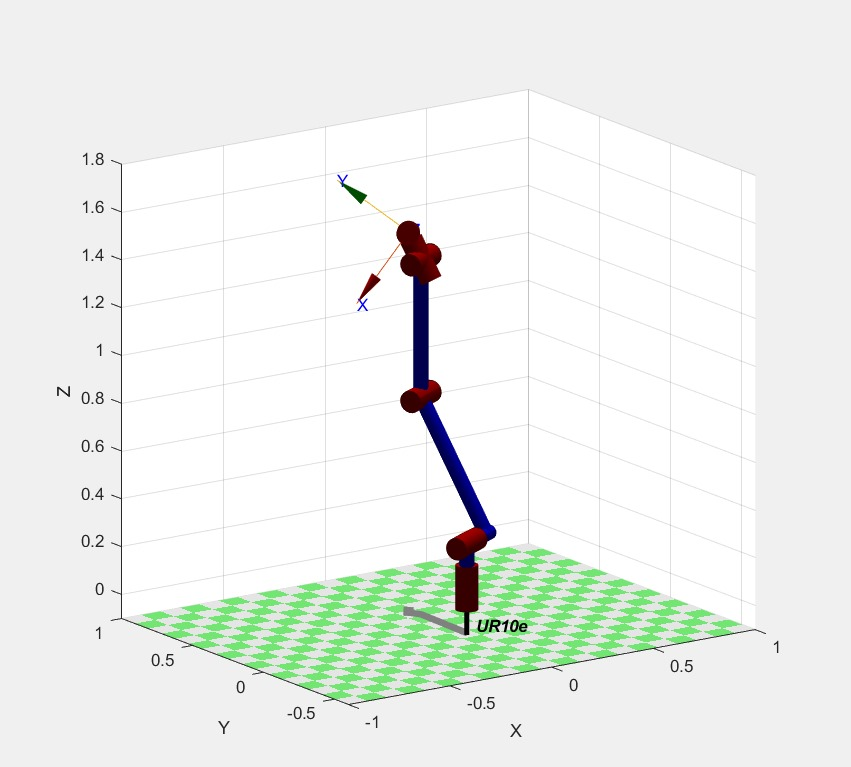
\includegraphics{1.jpeg}}
    \end{adjustbox}
    \caption{Verificación definición del robot 1.}
\end{figure}

\begin{figure}[H]
    \centering
    \begin{adjustbox}{scale = 0.45, max width=\columnwidth}
        \framebox{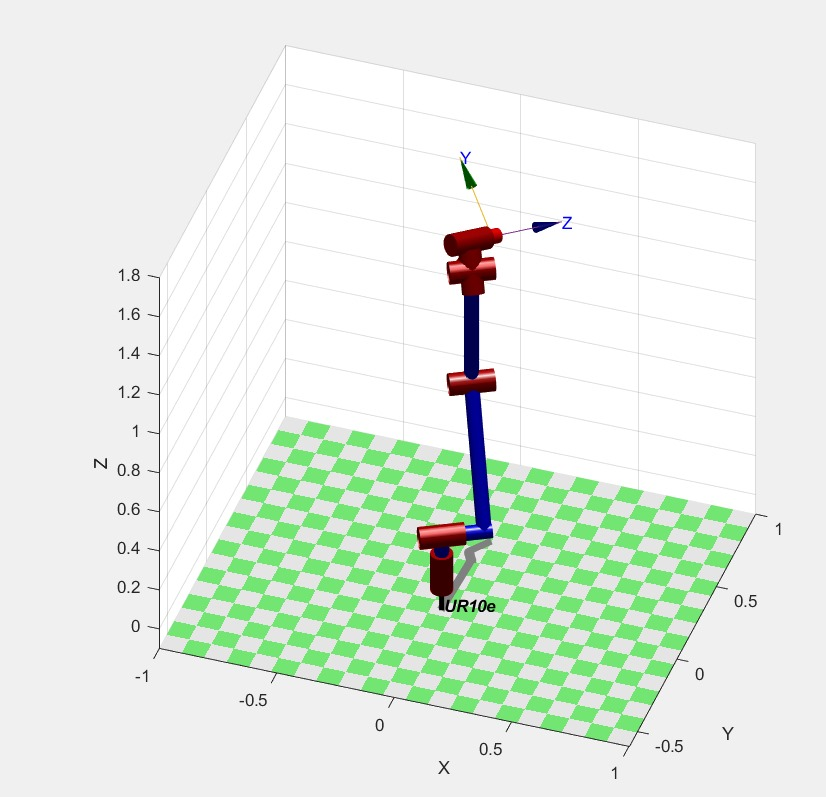
\includegraphics{2.jpeg}}
    \end{adjustbox}
    \caption{Verificación definición del robot 2.}
\end{figure}

\begin{figure}[H]
    \centering
    \begin{adjustbox}{scale = 0.45, max width=\columnwidth}
        \framebox{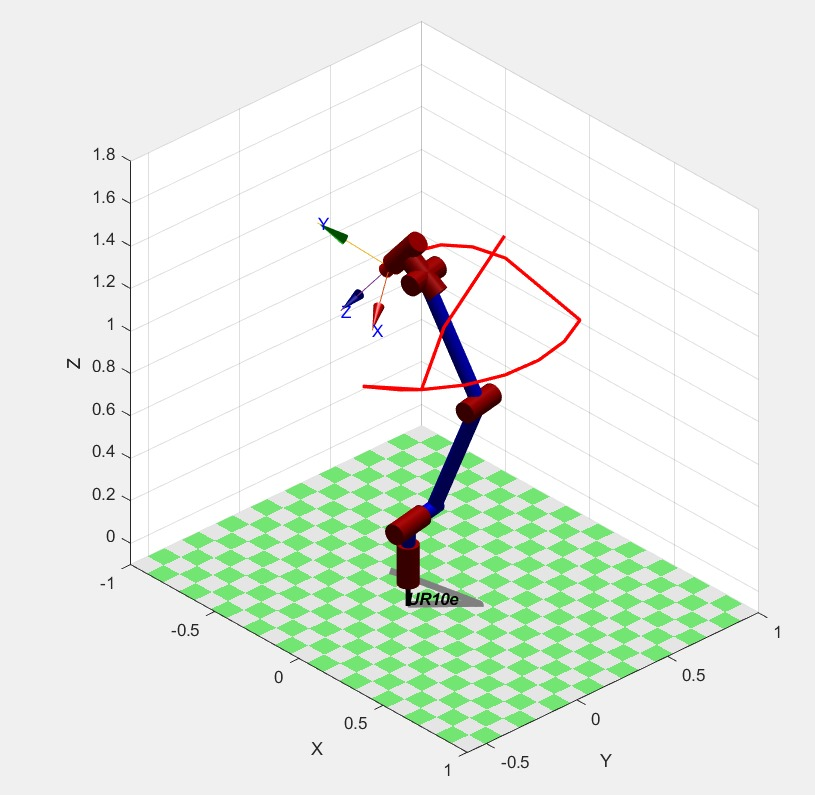
\includegraphics{3.jpeg}}
    \end{adjustbox}
    \caption{Verificación definición del robot 3 - Trayectoria.}
\end{figure}

\section{Ejercicio 2}
El archivo que muestra la definición de los sistemas (frames) para cada eslabón de la cadena
cinemática es \textbf{frames.m}.

\begin{itemize}
    \item Se incorpora la transformación de la \textbf{base} y de la \textbf{herramienta}.
\end{itemize}

\begin{figure}[H]
    \centering
    \begin{adjustbox}{scale = 0.6, max width=\columnwidth}
        \framebox{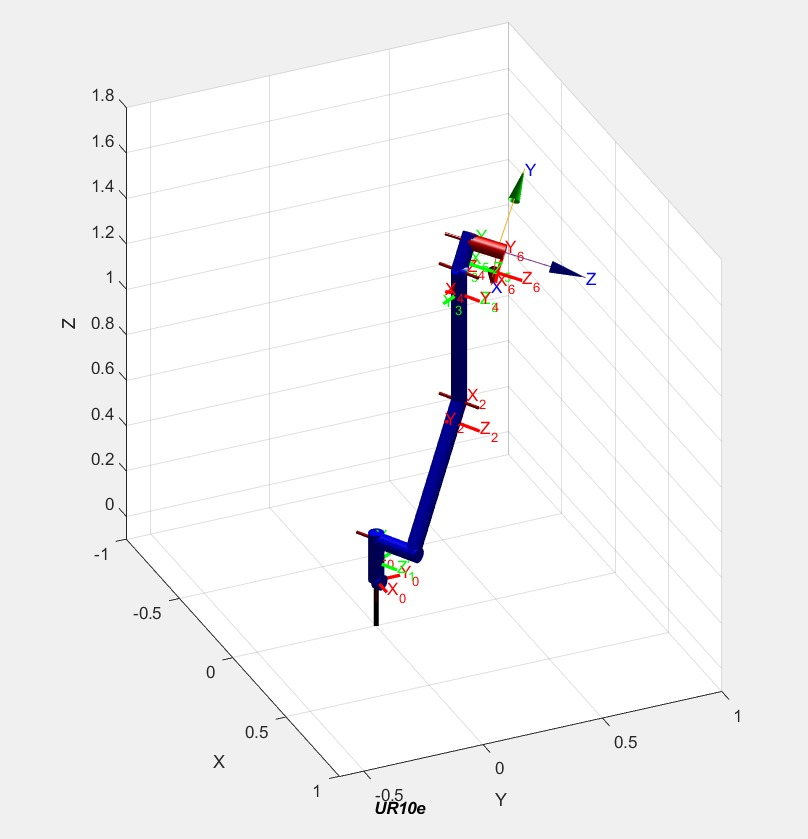
\includegraphics{4.jpeg}}
    \end{adjustbox}
    \caption{Frames 1}
\end{figure}

\begin{figure}[H]
    \centering
    \begin{adjustbox}{scale = 0.6, max width=\columnwidth}
        \framebox{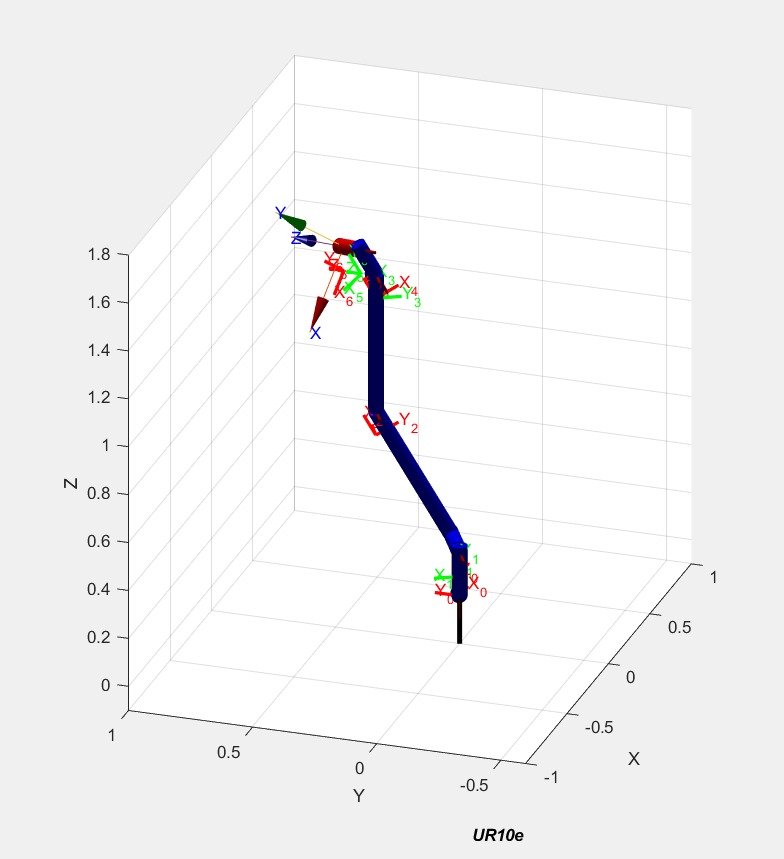
\includegraphics{5.jpeg}}
    \end{adjustbox}
    \caption{Frames 2}
\end{figure}
\end{document}